\let\lesson\undefined
\newcommand{\lesson}{\phantomlesson{Bài 15.}}
\setcounter{section}{2}
\section{Trắc nghiệm nhiều phương án lựa chọn}
\setcounter{ex}{0}
\Opensolutionfile{ans}[ans/VN10-Y24-PH-SYL-024P-TN]
% ===================================================================
\begin{ex}\mkstar{1}
Công cơ học là đại lượng	
	\choice
	{vô hướng, giá trị không âm}
	{vector, có thể âm, dương hoặc bằng 0}
	{vector, có giá trị không âm}
	{\True vô hướng, giá trị có thể âm, dương hoặc bằng 0}
	\loigiai{}
\end{ex}
% ===================================================================
\begin{ex}\mkstar{1}
	Trường hợp nào sau đây lực tác dụng không sinh công?
	\choice
	{\True Lực vuông góc với phương chuyển động của vật}
	{Lực cùng phương với phương chuyển động của vật}
	{Lực hợp với phương chuyển động một góc lớn hơn $\SI{90}{\degree}$}
	{Lực hợp với phương chuyển động một góc nhỏ hơn $\SI{90}{\degree}$}
	\loigiai{Khi lực vuông góc với phương chuyển động của vật thì $\alpha=\SI{90}{\degree}$, khi đó $\cos \alpha =0$, dẫn đến $A=Fs\cos \alpha=0$.}
\end{ex}	
% ===================================================================
	\begin{ex}\mkstar{1}
	Chọn nhận định \textbf{sai}.	
		\choice
		{Công của lực cản âm vì $\SI{90}{\degree} < \alpha <\SI{180}{\degree}$}
		{Công của lực phát động dương vì $\SI{90}{\degree} > \alpha >\SI{0}{\degree}$}
		{Vật dịch chuyển theo phương nằm ngang thì công của trọng lực bằng $0$}
		{\True Vật dịch chuyển trên mặt phẳng nghiêng thì công của trọng lực bằng $0$}
		\loigiai{Vật dịch chuyển trên mặt phẳng nghiêng thì công của trọng lực khác $0$, vì phương của trọng lực không vuông góc với phương của mặt nghiêng.}
	\end{ex}
% ===================================================================
\begin{ex}\mkstar{1}
	Dạng năng lượng \textbf{không} được thể hiện trong hình bên dưới là
	\begin{center}
		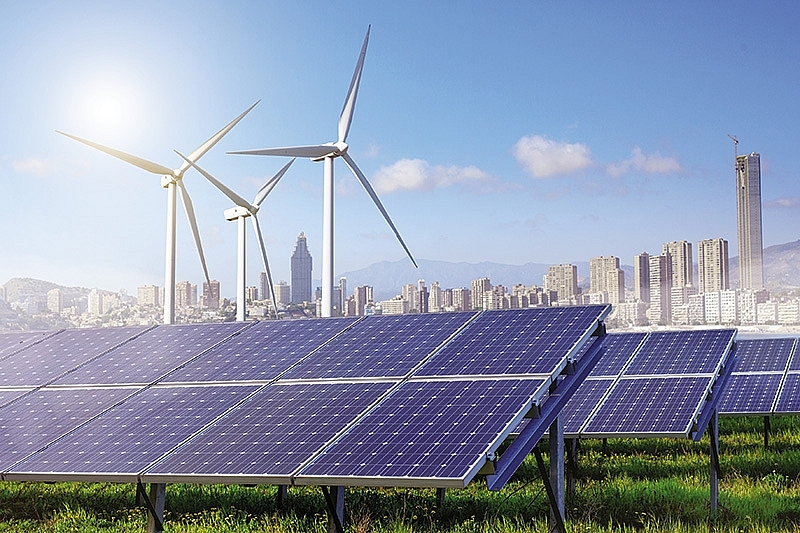
\includegraphics[width=0.4\linewidth]{../figs/VN10-2023-PH-TP024-P-1}
	\end{center}
	\choice
	{điện năng}
	{quang năng}
	{cơ năng}
	{\True năng lượng sinh học}
	\loigiai{}
\end{ex}
% ===================================================================
\begin{ex}\mkstar{1}
	Phát biểu nào sau đây là \textbf{sai} khi nói về năng lượng?
	\choice
	{Năng lượng là một đại lượng vô hướng}
	{Năng lượng có thể chuyển hóa từ dạng này sang dạng khác}
	{Năng lượng luôn là một đại lượng bảo toàn}
	{\True Trong hệ SI, đơn vị của năng lượng là calo}
	\loigiai{}
\end{ex}
% ===================================================================
\begin{ex}\mkstar{1}
	Đơn vị nào sau đây là đơn vị của công?
	\choice
	{$\si{\newton/\meter}$}
	{\True $\si{\kilogram\cdot \meter^2/\second^2}$}
	{$\si{\newton/\second}$}
	{$\si{\kilogram\cdot\meter^2/\second}$}
	\loigiai{}
\end{ex}
% ===================================================================
\begin{ex}\mkstar{2}
Một lực $\vec{F}$ có độ lớn không đổi tác dụng vào một vật đang chuyển động với vận tốc $\vec{v}$ theo các phương khác nhau như hình bên dưới.
	\begin{center}
		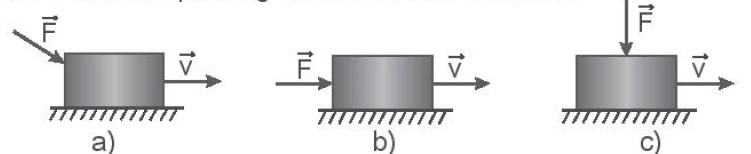
\includegraphics[width=0.4\linewidth]{../figs/VN10-2023-PH-TP024-P-5}
	\end{center}
	Độ lớn công do lực $F$ thực hiện xếp theo thứ tự tăng dần là
	\choice
	{(a), (b), (c)}
	{(a), (c), (b)}
	{(b), (a), (c)}
	{\True (c), (a), (b)}
	\loigiai{}
\end{ex}
% ===================================================================
\begin{ex}\mkstar{2}
Một người kéo một thùng gỗ trượt trên sàn nhà bằng một sợi dây hợp với phương ngang một góc $\SI{60}{\degree}$, lực tác dụng lên dây là $\SI{200}{N}$. Khi thùng gỗ được kéo và trượt một đoạn $\SI{10}{m}$ thì công của lực kéo là	
	\choice
	{$\SI{200}{J}$}
	{\True $\SI{1000}{J}$}
	{$\SI{2000}{J}$}
	{$\SI{120000}{J}$}
	\loigiai{Công của lực kéo:
		$$A=Fs\cos \alpha = \SI{1000}{J}.$$}
\end{ex}	

% ===================================================================
\begin{ex}\mkstar{2}
Người ta kéo một cái thùng nặng $\SI{20}{kg}$ trượt trên sàn nhà bằng một sợi dây hợp với phương nằm ngang một góc $\SI{60}{\degree}$, lực tác dụng lên dây là $\SI{300}{N}$. Tính công của lực đó khi thùng trượt được $\SI{10}{m}$. 	
	\choice
	{$\SI{1000}{J}$}
	{$\SI{500}{J}$}
	{\True $\SI{1500}{J}$}
	{$\SI{100}{J}$}
	\loigiai{Công của lực $F$ kéo thùng đi được $\SI{10}{m}$ là
		$$A = Fs\cos \alpha = \SI{1500}{J}.$$}
\end{ex}

% ===================================================================
\begin{ex}\mkstar{2}
Tác dụng lực không đổi $\SI{150}{N}$ theo phương hợp với phương ngang góc $\SI{30}{\degree}$ vào vật khối lượng $\SI{80}{kg}$ làm vật chuyển động được quãng $\SI{20}{m}$. Công của lực tác dụng có giá trị là	
	\choice
	{\True $\SI{2598}{J}$}
	{$\SI{598}{J}$}
	{$\SI{298}{J}$}
	{$\SI{258}{J}$}
	\loigiai{Công của lực tác dụng	
		$$A=Fs\cos \alpha =\SI{2598}{J}.$$}
\end{ex}
\Closesolutionfile{ans}
\section{Trắc nghiệm đúng/sai}
\setcounter{ex}{0}
\Opensolutionfile{ans}[ans/VN10-Y24-PH-SYL-024P-TF]
% ===================================================================
\begin{ex}\mkstar{1}
	Nhận định tính đúng/sai của các phát biểu sau khi nói về công của lực tác dụng lên vật.
	\choiceTF[t]
	{\True Vật rơi tự do thì trọng lực tác dụng lên vật sinh công dương}
	{Khi vật trượt lên mặt phẳng nghiêng thì lực ma sát giữa vật và mặt nghiêng sinh công dương}
	{Cần cẩu nâng đều khối vật liệu lên tòa nhà cao tầng thì trọng lực không thực hiện công}
	{Khi xe chuyển động chậm dần thì lực kéo của động cơ sinh công âm}
	\loigiai{}
\end{ex}
% ===================================================================
\begin{ex}\mkstar{3}
	Một cái thùng $\SI{50}{\kilogram}$ được đẩy lên $\SI{6.0}{\meter}$ theo mặt phẳng nghiêng góc $\SI{30}{\degree}$ với tốc độ  không đổi bởi một lực $\vec{F}$ không đổi như hình. Hệ số ma sát trượt giữa thùng và mặt nghiêng là $0,20$. Biết $\mathrm{AM}=\mathrm{MB}$.
	\begin{center}
		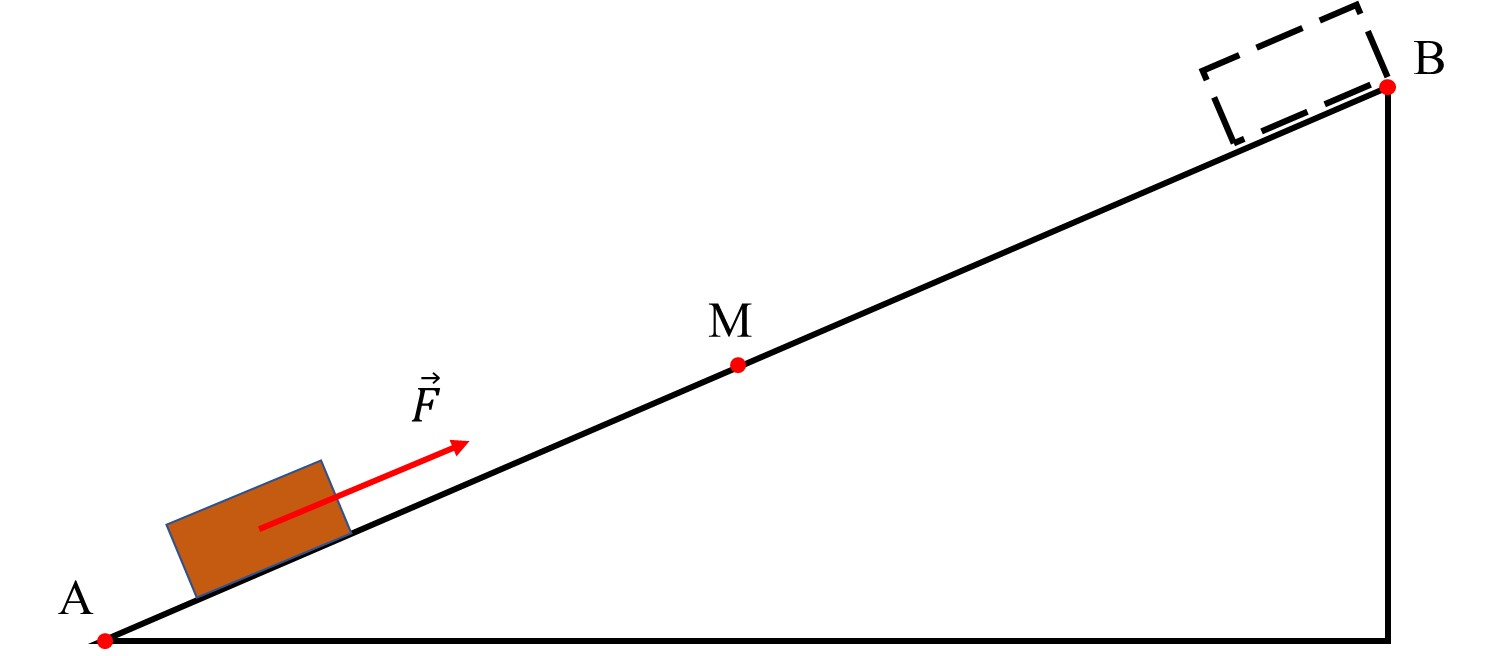
\includegraphics[width=0.5\linewidth]{../figs/VN10-2023-PH-TP024-P-8}
	\end{center}
	\choiceTF[t]
	{Công của trọng lực tác dụng lên thùng là công phát động}
	{Công của lực ma sát tác dụng lên thùng trên đoạn AM có giá trị lớn hơn trên đoạn AB}
	{Công của phản lực bằng công của trọng lực}
	{Độ lớn công của lực kéo bằng tổng độ lớn công của trọng lực và độ lớn công của lực ma sát}
	\loigiai{}
\end{ex}
\Closesolutionfile{ans}
\section{Tự luận}
\setcounter{ex}{0}
\Opensolutionfile{ans}[ans/VN10-Y24-PH-SYL-024P-TL]
% ======================================================================
\begin{ex}\mkstar{1}
Mỗi tế bào cơ trong cơ thể người có thể coi như một động cơ siêu nhỏ, khi con người hoạt động, tế bào cơ sử dụng năng lượng hoá học để thực hiện công. Trong mỗi nhịp hoạt động, tế bào cơ có thể sinh một lực $\SI{1.5E-12}{\newton}$ để dịch chuyển $\SI{8}{\nano\meter}$. Tính công mà tế bào cơ sinh ra trong mỗi nhịp hoạt động.	
	\loigiai{$A=\SI{1.2E-20}{\joule}$}
\end{ex}
% ======================================================================
\begin{ex}\mkstar{2}
		Một hành khách kéo đều một vali đi trong nhà ga trên sân bay trên quãng đường dài $\SI{150}{m}$ với lực kéo có độ lớn $\SI{40}{N}$ theo hướng hợp với phương ngang một góc $\SI{60}{\degree}$. Hãy xác định công của lực kéo của người này.
	\loigiai{Công của lực kéo của người: $$A=Fs\cos \alpha = \SI{3000}{J}.$$}
\end{ex}
% ======================================================================
\begin{ex}\mkstar{2}
	Một thùng nước khối lượng $\SI{10}{kg}$ được kéo cho chuyển động thẳng đều lên cao $\SI{5}{m}$ trong thời gian 1 phút 40 giây. Tính công của lực kéo. Lấy $g=\SI{10}{m/s^2}$.
	\loigiai{Lực kéo thùng nước để thùng chuyển động thẳng đều:
		$$F=P=mg=\SI{100}{N}.$$
		Công của lực kéo:
		$$A=Fs=\SI{500}{J}.$$}
\end{ex}
% ======================================================================
\begin{ex}\mkstar{2}
	Khi kiểm tra gầm xe ô tô, người ta sử dụng máy nâng ô tô lên độ cao $h = \SI{160}{cm}$ so với mặt sàn. Cho biết khối lượng ô tô là $m = \text{1,5}\ \text{tấn}$. Lấy gia tốc trọng trường $g=\SI{10}{\meter/\second^2}$. Tính công tối thiểu mà máy nâng đã thực hiện.
	\begin{center}
		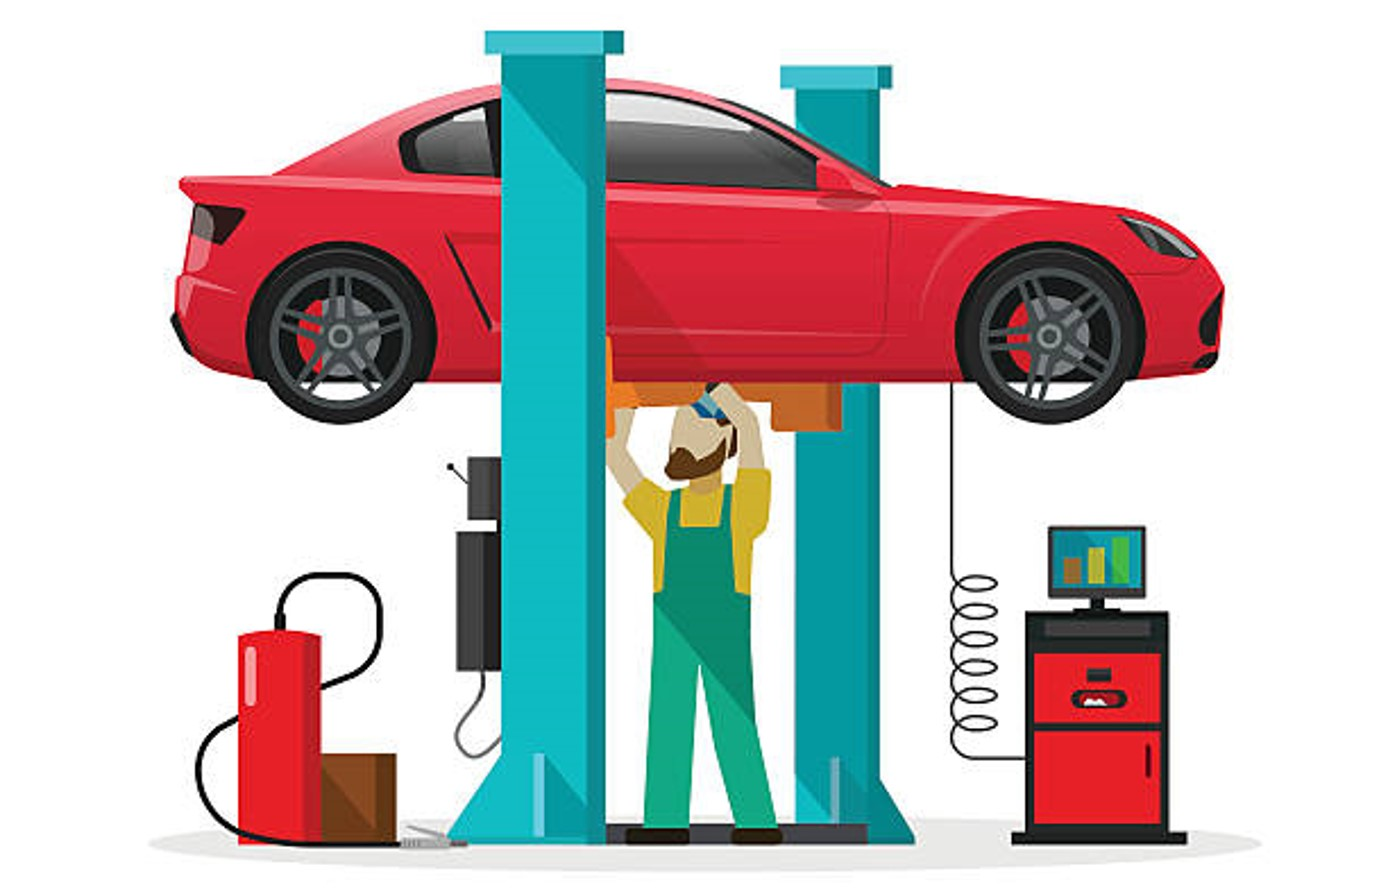
\includegraphics[width=0.3\linewidth]{../figs/VN10-2023-PH-TP024-P-2}
	\end{center}
	\loigiai{Để nâng được ô tô thì máy nâng phải tác dụng vào ô tô một lực có độ lớn tối thiểu bằng trọng lượng của ô tô:
		$$F = P =mg =\SI{1.5E4}{\newton}.$$
	Công tối thiểu mà máy nâng đã thực hiện là:
		$$A = Ph = \SI{24000}{J} = \SI{24}{kJ}.$$}
\end{ex}
% ======================================================================
\begin{ex}\mkstar{2}
	Một kĩ sư xây dựng nặng $\SI{75}{\kilogram}$ trèo lên một chiếc thang dài $\SI{2.75}{\meter}$. Thang được dựa vào bức tường thẳng đứng và tạo một góc $\alpha=\SI{75}{\degree}$ với mặt phẳng ngang.
	\begin{center}
		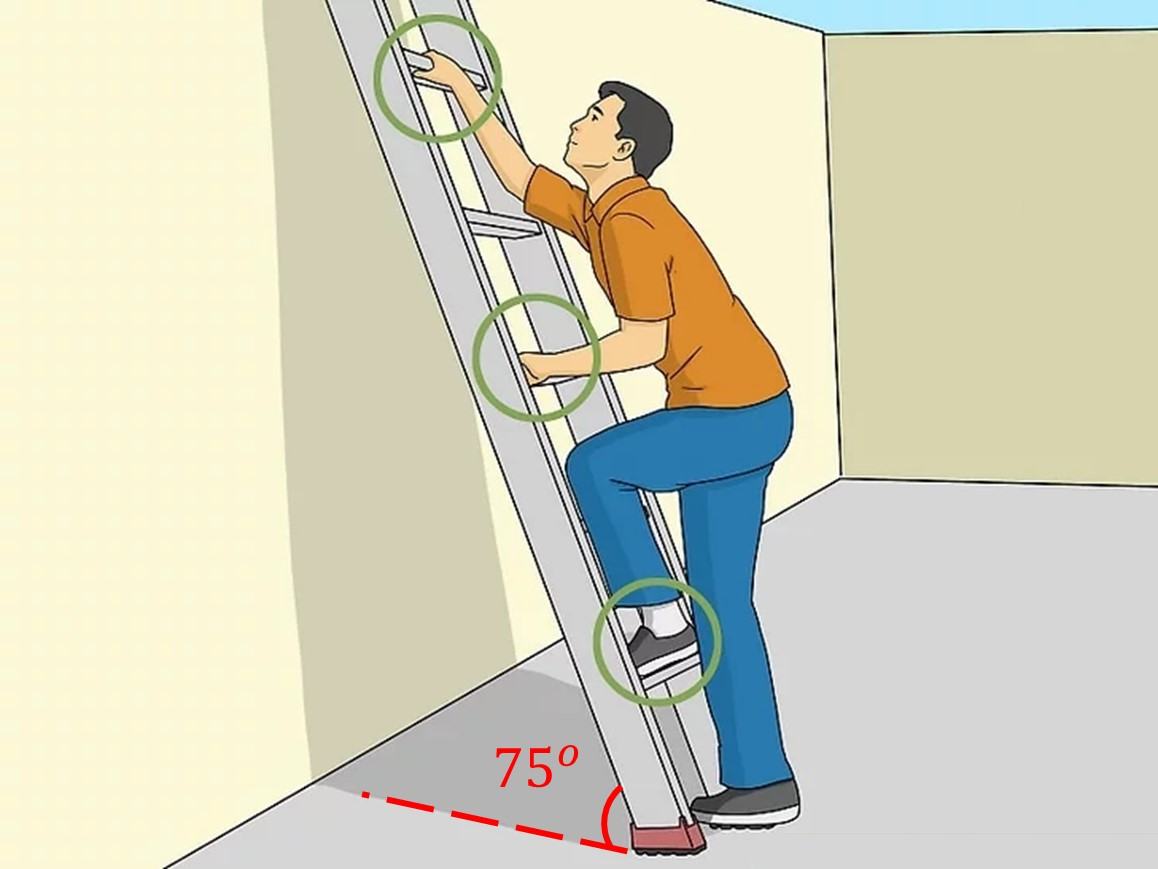
\includegraphics[width=0.4\linewidth]{../figs/VN10-2023-PH-TP024-P-3}
	\end{center}
	\begin{enumerate}[label=\alph*)]
		\item Tính công của trọng lực tác dụng lên kĩ sư khi người này leo từ chân đến đỉnh thang.
		\item Đáp án của câu a có phụ thuộc vào tốc độ của người kĩ sư trong quá trình leo không?
	\end{enumerate}
	\loigiai{
\begin{enumerate}[label=\alph*)]
	\item $$A_P=-mg\ell\sin\alpha\approx\SI{-1992.2}{\joule}.$$
	\item Không phụ thuộc vào tốc độ của người kĩ sư trong quá trình leo.
\end{enumerate}
	}
\end{ex}
% ======================================================================
\begin{ex}\mkstar{3}
	Một người y tá đẩy bệnh nhân nặng $\SI{87}{\kilogram}$ trên chiếc xe băng ca nặng $\SI{18}{\kilogram}$ làm cho bệnh nhân và xe băng ca chuyển động thẳng trên mặt sàn nằm ngang với gia tốc không đổi là $\SI{0.55}{\meter/\second^2}$. Bỏ qua ma sát giữa bánh xe và mặt sàn.
	\begin{center}
		
\includegraphics[width=0.4\linewidth]{../figs/VN10-2023-PH-TP024-P-6}
	\end{center}
	\begin{enumerate}[label=\alph*)]
		\item Tính công mà y tá đã thực hiện khi bệnh nhân và xe băng ca chuyển động được $\SI{1.9}{\meter}$.
		\item Sau quãng đường dài bao nhiêu thì y tá sẽ tiêu hao một công là $\SI{140}{\joule}$?
	\end{enumerate}
	\loigiai{
	\begin{enumerate}[label=\alph*)]
		\item $F=(m+m')a=\SI{57.75}{\newton}$.
		\item $s'=\dfrac{A'}{F}=\SI{2.4}{\meter}$.
	\end{enumerate}
	}
\end{ex}
% ======================================================================
\begin{ex}\mkstar{3}
	Một ô tô có khối lượng $m=\SI{1.30E3}{\kilogram}$ di chuyển trên đoạn đường ABCD có dạng như hình bên dưới, trong đó BC là đoạn đường nằm ngang ở độ cao $h=\SI{50.0}{\meter}$ so với mặt phẳng ngang chứa AD. Biết rằng $\text{BC}=\SI{20}{\kilo\meter}$, gia tốc rơi tự do $g=\SI{9.80}{\meter/\second^2}$, độ dài các cung cong nối các đoạn đường thẳng với nhau rất nhỏ so với chiều dài của các đoạn thẳng đó, hãy tính công của trọng lực trên các đoạn đường AB, BC, CD.
	\begin{center}
		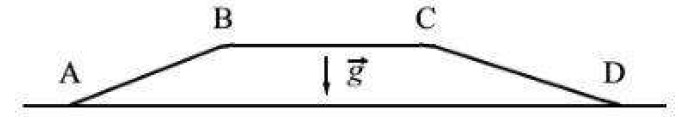
\includegraphics[width=0.4\linewidth]{../figs/VN10-2023-PH-TP024-P-7}
	\end{center}
	\loigiai{
	$A_{\mathrm{AB}}=-mgh=\SI{-637}{\kilo\joule}$; $A_{\mathrm{BC}}=0$; $A_{\mathrm{CD}}=mgh=\SI{637}{\kilo\joule}$.}
\end{ex}
% ======================================================================
\begin{ex}\mkstar{3}
Một chiếc đàn piano có khối lượng $\SI{380}{\kilogram}$ được giữ cho trượt đều xuống một đoạn dốc dài $\SI{2.9}{\meter}$, nghiêng một góc $\SI{10}{\degree}$ so với phương ngang. Biết lực do người tác dụng có phương song song với mặt phẳng nghiêng như hình bên dưới. 
\begin{center}
	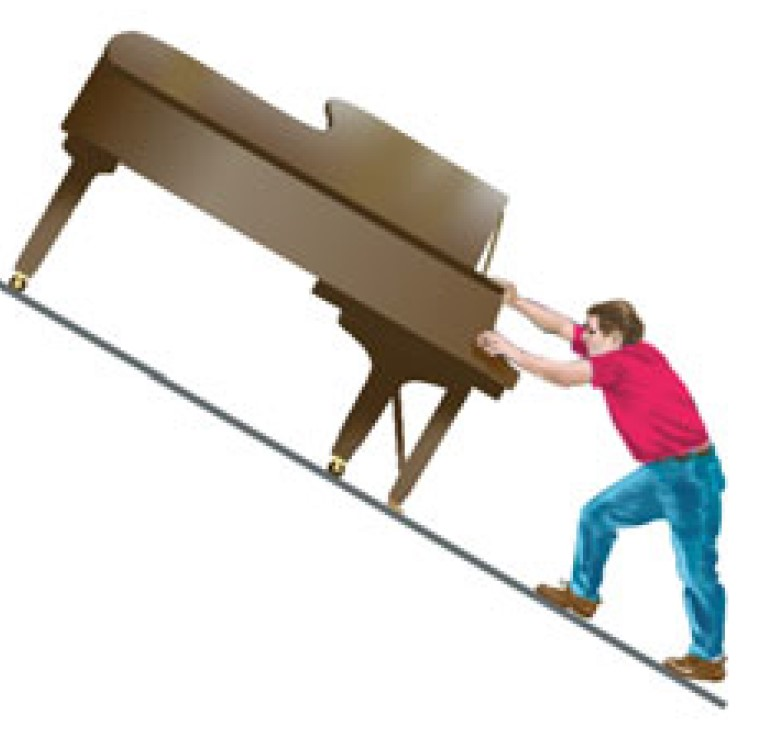
\includegraphics[width=0.35\linewidth]{../figs/VN10-2023-PH-TP024-P-4}
\end{center}
Bỏ qua mọi ma sát. Lấy $g=\SI{9.8}{\meter/\second^2}$. Hãy xác định:
\begin{enumerate}[label=\alph*)]
	\item lực do người tác dụng lên đàn piano.
	\item công của lực do người tác dụng lên đàn piano.
	\item công của trọng lực tác dụng lên đàn piano.
	\item tổng công của tất cả các lực tác dụng lên đàn piano.
\end{enumerate}
	\loigiai{
	\begin{enumerate}[label=\alph*)]
		\item $F=mg\sin\alpha\approx\SI{646.67}{\newton}$.
		\item Công do người này thực hiện: $A_{\vec{F}}=Fd\cos\theta\approx\SI{-1875.33}{\joule}$.
		\item Công của trọng lực: $A_{\vec{P}}=mgd\cos\left(\SI{90}{\degree}-\alpha\right)\approx\SI{1875.33}{\joule}.$
		\item Tổng công thực hiện lên đàn piano: $A=A_{\vec{F}}+A_{\vec{P}}+A_{\vec{N}}=0.$
	\end{enumerate}
	}
\end{ex}
% ======================================================================
\begin{ex}\mkstar{3}
	Một khối gỗ có trọng lượng là $P=\SI{50}{\newton}$ được đẩy trượt đều lên trên một mặt phẳng nghiêng nhẵn với góc nghiêng $\SI{25}{\degree}$ so với phương ngang. Biết khối gỗ di chuyển được một đoạn $\SI{1}{\meter}$ trên mặt phẳng nghiêng. Tìm công mà người đẩy thực hiện trên khối gỗ nếu lực tác dụng:
	\begin{enumerate}[label=\alph*)]
		\item song song với mặt phẳng nghiêng.
		\item song song với mặt phẳng ngang.
	\end{enumerate}
	\loigiai{
	\begin{enumerate}[label=\alph*)]
		\item $A_{\vec{F}}=Pd\sin\SI{25}{\degree}\approx\SI{21.13}{\joule}$.
		\item $A_{\vec{F}}=Pd\tan\SI{25}{\degree}\approx\SI{23.32}{\joule}$.
	\end{enumerate}
	}
\end{ex}
% ======================================================================
\begin{ex}\mkstar{3}
Một người dùng lực $F$ hợp với phương nằm ngang một góc $\alpha=\SI{60.0}{\degree}$ để kéo vật có khối lượng $m=\SI{50.0}{\kilogram}$ trượt trên mặt sàn nằm ngang một đoạn thẳng có độ dài $s=\SI{10.0}{\meter}$ với tốc độ không đổi. Biết hệ số ma sát giữa vật và mặt sàn là $\mu=0,250$; thành phần thẳng đứng của lực $F$ hướng từ dưới lên trên, gia tốc rơi tự do $g=\SI{9.8}{\meter/\second^2}$. Tính:	
\begin{enumerate}[label=\alph*)]
	\item công của trọng lực.
	\item công của lực $F$.
	\item công của lực ma sát.
\end{enumerate}
	\loigiai{
	\begin{enumerate}[label=\alph*)]
		\item $A_{\vec{P}}=0$.
		\item Vật trượt đều nên:
		$$F\cos\SI{60}{\degree}=F_{\text{ms}}=\mu\left(mg-F\sin\SI{60}{\degree}\right)\Rightarrow F\approx\SI{171}{\newton}.$$
		Công của lực $\vec{F}$:		
		$A_{\vec{F}}=Fs\cos\SI{60}{\degree}\approx\SI{855}{\joule}$.
		\item Công của lực ma sát:
		$A_{\vec{F}_{\text{ms}}}=F_{\text{ms}}s\cos\SI{180}{\degree}=-F\cos\SI{60}{\degree}s\approx\SI{-855}{\joule}$.
	\end{enumerate}
	}
\end{ex}
% ======================================================================
\begin{ex}\mkstar{3}
	Một ngưởi dùng lực $F$ hợp với phương nằm ngang một góc $\alpha=\SI{30.0}{\degree}$ để đẩy vật có khối lượng $m=\SI{50.0}{\kilogram}$ trượt trên mặt sàn nằm ngang một đoạn thẳng có độ dài $s=\SI{15.0}{\meter}$ với vận tốc không đổi. Biết hệ số ma sát giữa vật và mặt sàn là $\mu=0,30$, thành phần thẳng đứng của $F$ hướng từ trên xuống dưới, gia tốc rơi tự do $g=\SI{9.8}{\meter/\second^2}$. Tính:
	\begin{enumerate}[label=\alph*)]
		\item công của trọng lực.
		\item công của lực $F$.
		\item công của lực ma sát.
	\end{enumerate}
	\loigiai{
	\begin{enumerate}[label=\alph*)]
		\item Công của trọng lực $A_{\vec{P}}=0$.
		\item Vì vật chuyển động thẳng đều nên:
		$$F\cos\alpha=\mu\left(mg+F\sin\alpha\right)\Rightarrow F\approx\SI{205.3}{\newton}.$$
		Công của lực $\vec{F}$:
		$$A_{\vec{F}}=Fs\cos\SI{30}{\degree}\approx\SI{2667}{\joule}.$$
		\item Công của lực ma sát:
		$$A_{\vec{F}_{\text{ms}}}=F_{\text{ms}}s\cos\SI{180}{\degree}=-F\cos\SI{30}{\degree}s\approx\SI{-2667}{\joule}.$$
	\end{enumerate}
	}
\end{ex}
\Closesolutionfile{ans}